\subsection{Learning $\nfhef$}

We now describe a learning algorithm for $\nfhef$.
Our algorithm is based on Angluin's $L^*$ algorithm \cite{Angluin87} for regular languages, and aims to learn a minimal deterministic permutation-sequence complete $\nfhef$ with a minimal number of variables for a hyperlanguage $\cal L$.

As with $L^*$, our algorithm consists of two entities: a {\em learner} and a {\em teacher}.
During the learning process, the learner asks the teacher two types of queries: {\em membership queries} (``is the hyperword $S$ in $\cal L$?'') and {\em equivalence queries} (``Is $\A$ an $\nfhef$ for $\cal L$?'').


The number of variables, as well as the quantification condition $\alpha$, is unknown to the learner in advance, and is established during the learning procedure. 
In every step, the learner may cause one of the following to occur in the $\nfhef$ $\A$ that it maintains:
\begin{enumerate}
    \item Increase the number of states;
    \item Increase the number of variables;
    \item Turn an $\exists$ quantifier to a $\forall$ quantifier.
\end{enumerate}

As with $L^*$, the learner maintains an {\em observation table} $T$, which, intuitively, maintains the states and transitions of the underlying automaton that have been learned so far. In addition, the learner maintains the current number of variables $k$ (which also influences the alphabet of the observation table), and the number of $\exists$ quantifiers $t$ in the quantification condition. 

In case of a failed equivalence query, the teacher returns a {\em counterexample}: a {\em negative counterexample} is a hyperword that is not in $\lang{\A}$ and is in $\cal L$, and a {\em positive counterexample} is a hyperword that is in $\lang{\A}$, but is not in $\cal L$. We assume that the teacher always returns a minimal counterexample (in terms of set size).

The actions of the learner depend on the properties of the returned counterexample $S$ it gets from the teacher. 
We say that $S$ is {\em manifested} in $T$ if there exists a word $w$ in $T$ that is formed by zipping the words in $S$ in some order.
\begin{enumerate}
    \item 
    If $S$ is a positive counterexample of size $k$ or less, that is not manifested in $T$, then the learner adds  $\zip(S)$ to $T$, where $\zip(S)$ denotes zipping the words in $S$ in some arbitrary order. 
    \item 
    If $S$ is a positive counterexample of size $k$ or less, that is manifested in $T$, then the learner sets $t\leftarrow t-1$. 
    \item
    If $S$ is a positive counterexample of size $k'>k$, then the learner replaces every letter $\sigma$ in the transitions with $\uparrow^{k'}(\sigma)$, and sets $t\leftarrow t+(k'-k)$. 
    \item If $S$ is a negative counterexample, and $k>t$. then it must be that $S$ is of size $k$ or less, and does not already appear in $T$. The learner then adds $S$ to $T$.
    \item if $S$ is a negative counterexample of size $k'>k$, and $k=t$ (that is, the quantifiers are all $\exists$), then the learner sets $t\leftarrow t-1$.  
\end{enumerate}




\begin{figure} 

\centering


\tikzset{every picture/.style={line width=0.75pt}} %set default line width to 0.75pt        

\scalebox{.95}{
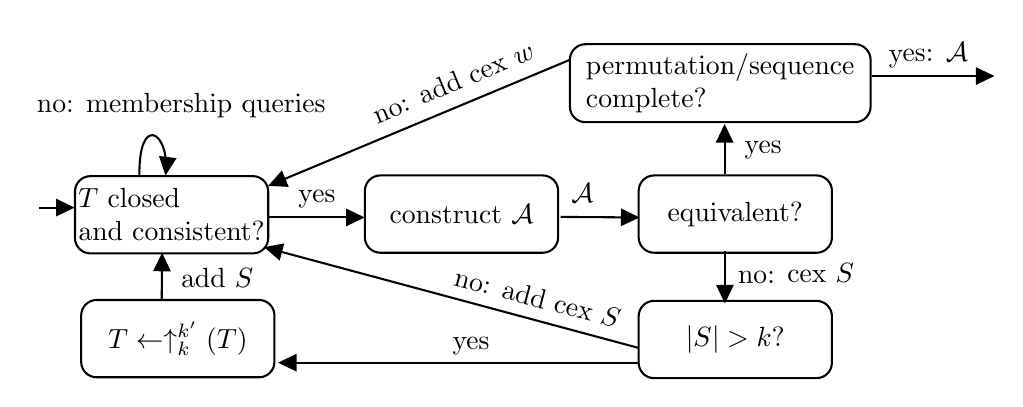
\begin{tikzpicture}[x=0.75pt,y=0.75pt,yscale=-1,xscale=1]
%uncomment if require: \path (0,427.3333320617676); %set diagram left start at 0, and has height of 427.3333320617676

%Curve Lines [id:da3242324591734014] 
\draw    (78.05,195.76) .. controls (77.68,166.57) and (91.81,174.17) .. (90.87,193.02) ;
\draw [shift={(90.63,195.76)}, rotate = 276.98] [fill={rgb, 255:red, 0; green, 0; blue, 0 }  ][line width=0.08]  [draw opacity=0] (8.93,-4.29) -- (0,0) -- (8.93,4.29) -- cycle    ;

%Rounded Rect [id:dp5230596682902247] 
\draw   (285.46,140.05) .. controls (285.46,135.9) and (288.82,132.53) .. (292.98,132.53) -- (422.81,132.53) .. controls (426.96,132.53) and (430.33,135.9) .. (430.33,140.05) -- (430.33,162.59) .. controls (430.33,166.74) and (426.96,170.11) .. (422.81,170.11) -- (292.98,170.11) .. controls (288.82,170.11) and (285.46,166.74) .. (285.46,162.59) -- cycle ;
%Straight Lines [id:da19996498797143802] 
\draw    (360,195) -- (360,174) ;
\draw [shift={(360,171)}, rotate = 450] [fill={rgb, 255:red, 0; green, 0; blue, 0 }  ][line width=0.08]  [draw opacity=0] (8.93,-4.29) -- (0,0) -- (8.93,4.29) -- cycle    ;

%Straight Lines [id:da7742261006504376] 
\draw    (360.15,232.33) -- (360.15,254.42) ;
\draw [shift={(360.15,257.42)}, rotate = 270] [fill={rgb, 255:red, 0; green, 0; blue, 0 }  ][line width=0.08]  [draw opacity=0] (8.93,-4.29) -- (0,0) -- (8.93,4.29) -- cycle    ;

%Straight Lines [id:da7240079665223356] 
\draw    (318.59,285.97) -- (147.88,285.97) ;
\draw [shift={(144.88,285.97)}, rotate = 360] [fill={rgb, 255:red, 0; green, 0; blue, 0 }  ][line width=0.08]  [draw opacity=0] (8.93,-4.29) -- (0,0) -- (8.93,4.29) -- cycle    ;

%Straight Lines [id:da4355292395155117] 
\draw    (88.79,255.9) -- (88.97,236) ;
\draw [shift={(89,233)}, rotate = 450.53] [fill={rgb, 255:red, 0; green, 0; blue, 0 }  ][line width=0.08]  [draw opacity=0] (8.93,-4.29) -- (0,0) -- (8.93,4.29) -- cycle    ;

%Straight Lines [id:da9395518765143251] 
\draw    (140,216) -- (183.56,216) ;
\draw [shift={(186.56,216)}, rotate = 180] [fill={rgb, 255:red, 0; green, 0; blue, 0 }  ][line width=0.08]  [draw opacity=0] (8.93,-4.29) -- (0,0) -- (8.93,4.29) -- cycle    ;

%Straight Lines [id:da9876991440040634] 
\draw    (280.98,215.74) -- (316,215.98) ;
\draw [shift={(319,216)}, rotate = 180.4] [fill={rgb, 255:red, 0; green, 0; blue, 0 }  ][line width=0.08]  [draw opacity=0] (8.93,-4.29) -- (0,0) -- (8.93,4.29) -- cycle    ;

%Straight Lines [id:da8894863053773812] 
\draw    (318.59,278.87) -- (141.02,231.11) ;
\draw [shift={(138.12,230.33)}, rotate = 375.05] [fill={rgb, 255:red, 0; green, 0; blue, 0 }  ][line width=0.08]  [draw opacity=0] (8.93,-4.29) -- (0,0) -- (8.93,4.29) -- cycle    ;

%Rounded Rect [id:dp7304454638728446] 
\draw   (318.59,203.21) .. controls (318.59,199.09) and (321.93,195.76) .. (326.04,195.76) -- (404.26,195.76) .. controls (408.37,195.76) and (411.71,199.09) .. (411.71,203.21) -- (411.71,225.56) .. controls (411.71,229.67) and (408.37,233) .. (404.26,233) -- (326.04,233) .. controls (321.93,233) and (318.59,229.67) .. (318.59,225.56) -- cycle ;
%Straight Lines [id:da989641097303189] 
\draw    (285.46,140.05) -- (142.89,199.6) ;
\draw [shift={(140.12,200.76)}, rotate = 337.33000000000004] [fill={rgb, 255:red, 0; green, 0; blue, 0 }  ][line width=0.08]  [draw opacity=0] (8.93,-4.29) -- (0,0) -- (8.93,4.29) -- cycle    ;

%Straight Lines [id:da5782151978812646] 
\draw    (431,147.86) -- (487,147.86) ;
\draw [shift={(490,147.86)}, rotate = 180] [fill={rgb, 255:red, 0; green, 0; blue, 0 }  ][line width=0.08]  [draw opacity=0] (8.93,-4.29) -- (0,0) -- (8.93,4.29) -- cycle    ;

%Rounded Rect [id:dp9174543196821443] 
\draw   (186.68,203.21) .. controls (186.68,199.09) and (190.02,195.76) .. (194.13,195.76) -- (272.35,195.76) .. controls (276.46,195.76) and (279.8,199.09) .. (279.8,203.21) -- (279.8,225.56) .. controls (279.8,229.67) and (276.46,233) .. (272.35,233) -- (194.13,233) .. controls (190.02,233) and (186.68,229.67) .. (186.68,225.56) -- cycle ;
%Rounded Rect [id:dp013423076978946291] 
\draw   (318.59,263.62) .. controls (318.59,259.51) and (321.93,256.17) .. (326.04,256.17) -- (404.26,256.17) .. controls (408.37,256.17) and (411.71,259.51) .. (411.71,263.62) -- (411.71,285.97) .. controls (411.71,290.08) and (408.37,293.42) .. (404.26,293.42) -- (326.04,293.42) .. controls (321.93,293.42) and (318.59,290.08) .. (318.59,285.97) -- cycle ;
%Rounded Rect [id:dp7630850927481354] 
\draw   (47.01,203.54) .. controls (47.01,199.42) and (50.35,196.09) .. (54.46,196.09) -- (132.68,196.09) .. controls (136.79,196.09) and (140.12,199.42) .. (140.12,203.54) -- (140.12,225.89) .. controls (140.12,230) and (136.79,233.33) .. (132.68,233.33) -- (54.46,233.33) .. controls (50.35,233.33) and (47.01,230) .. (47.01,225.89) -- cycle ;
%Rounded Rect [id:dp6612685395327704] 
\draw   (50,263.2) .. controls (50,259.09) and (53.34,255.76) .. (57.45,255.76) -- (135.67,255.76) .. controls (139.78,255.76) and (143.11,259.09) .. (143.11,263.2) -- (143.11,285.55) .. controls (143.11,289.66) and (139.78,293) .. (135.67,293) -- (57.45,293) .. controls (53.34,293) and (50,289.66) .. (50,285.55) -- cycle ;
%Straight Lines [id:da6707127407283302] 
\draw    (29.79,211.24) -- (43.84,211.24) ;
\draw [shift={(46.84,211.24)}, rotate = 180] [fill={rgb, 255:red, 0; green, 0; blue, 0 }  ][line width=0.08]  [draw opacity=0] (8.93,-4.29) -- (0,0) -- (8.93,4.29) -- cycle    ;


% Text Node
\draw (141.81,182.12) node   [align=left] {$ $};
% Text Node
\draw (93.57,214.71) node   [align=left] {$\displaystyle T${\fontfamily{ptm}\selectfont  }~closed \\and consistent?};
% Text Node
\draw (98.22,162.32) node   [align=left] {no: membership queries};
% Text Node
\draw (233.24,214.38) node   [align=left] {construct $\displaystyle \mathcal{A}$};
% Text Node
\draw (357.89,151.32) node   [align=left] {permutation/sequence \\complete?};
% Text Node
\draw (229.13,150.68) node  [rotate=-337.24] [align=left] {no: add cex~{\fontfamily{ptm}\selectfont  }$\displaystyle w$};
% Text Node
\draw (365.15,214.38) node   [align=left] {equivalent?};
% Text Node
\draw (394.44,242.91) node  [rotate=-359.45] [align=left] {no: cex $\displaystyle S$};
% Text Node
\draw (365.15,274.8) node  [rotate=-359.45] [align=left] {$\displaystyle |S| >k?$};
% Text Node
\draw (378.6,183.41) node  [rotate=-359.45] [align=left] {yes};
% Text Node
\draw (163.6,207.37) node  [rotate=-359.45] [align=left] {yes};
% Text Node
\draw (291.5,204) node   [align=left] {{\fontfamily{ptm}\selectfont  }$\displaystyle \mathcal{A}$};
% Text Node
\draw (269.92,254.66) node  [rotate=-14.77] [align=left] {no: add cex $\displaystyle S${\fontfamily{ptm}\selectfont  }};
% Text Node
\draw (237.84,277.89) node  [rotate=-359.61] [align=left] {yes};
% Text Node
\draw (458.14,137.71) node  [rotate=-359.45] [align=left] {yes: {\fontfamily{ptm}\selectfont  }$\displaystyle \mathcal{A}$};
% Text Node
\draw (115.57,245.15) node  [rotate=-359.61] [align=left] {add~{\fontfamily{ptm}\selectfont  }$\displaystyle S${\fontfamily{ptm}\selectfont  }};
% Text Node
\draw (96.56,274.38) node   [align=left] {{\fontfamily{ptm}\selectfont  }$\displaystyle T\leftarrow \uparrow ^{k'}_{k}( T)${\fontfamily{ptm}\selectfont  }};


\end{tikzpicture}
}

\caption{The learning process flow for $\nfhf$ and $\nfhe$.}
\label{fig:learning_flow}
\vspace{-3mm}
\end{figure}


